\documentclass[letterpaper, 11pt]{amsart}

\usepackage{fullpage}
\usepackage{graphicx}
\usepackage{amsmath, amssymb, amsfonts}

\usepackage{color}
\usepackage[colorlinks=true,linkcolor=red,citecolor=blue,urlcolor=cyan]{hyperref}

\definecolor{crimsonred}{RGB}{190,0,0}
\definecolor{granitepeak}{RGB}{117,142,153}
\definecolor{lakecolor}{RGB}{58,191,192}

\newcommand{\red}[1]{\textcolor{crimsonred}{#1}}
\newcommand{\DAR}[1]{\textcolor{granitepeak}{#1}}
\newcommand{\replace}[1]{\textcolor{lakecolor}{#1}}
\newcommand{\BO}[1]{\textcolor{blue}{\small {\sf BO:\@ #1}}}


\begin{document}
\noindent {\bf Bob Stutchbury \\ 
Math 5750/6880: Mathematics of Data Science \\  
Project \#1 Final Project \\  % when appropriate change me to Final Report
\today \\ }


%%%%%%%%%%%%%%%%%%%%%%%%%%%%%%%%%%
\section{\LaTeX}

\medskip

\noindent {\bf Experience.} I know a bit of the equation syntax, though not much of the document formatting stuff. As a computer nerd with opinions, I am forced to mention Typst, which is built on being a good markup language, as opposed to \LaTeX, which seems to largely survive on path dependence and spite.

%%%%%%%%%%%%%%%%%%%%%%%%%%%%%%%%%%
\section{GitHub}
My GitHub Project1 repository is located here (see projects/Project1 for this wd):
\begin{center}
\url{https://github.com/kerbs23/F25_math_for_data_science}
\end{center}



\medskip

\noindent {\bf Experience.} Used Git for keeping track of some personal projects, but I'm certainly no wizzard and no collaborative experience. Basic forking stuff on gh, but never studied it really.



%%%%%%%%%%%%%%%%%%%%%%%%%%%%%%%%%%
\section{Python and Google Colab}
I solved the following ProjectEuler problem: \url{https://projecteuler.net/problem=69}

\medskip

\noindent {\bf Solution.}
\noindent Used observations about how the score was connected to underlying prime factors to guess 510510, which a brute force run through showed to be correct.

\medskip

\noindent {\bf Experience.} Self-taught data science stuff by way of getting hired to do it before I was really qualified (Research econometrecs; so data cleaning, static analysis, fixed-effect regression and event study (staggered and no) causal type stuff), so my CS fundamentals arn't great but trying to improve.
A bit more reliant on AI than I am proud to admit, but also working on that.



%%%%%%%%%%%%%%%%%%%%%%%%%%%%%%%%%%
\section{Regression Analysis}

\subsection{Dataset Description}
The California Housing dataset contains median house values for California districts (with a cap) along with eight predictor variables:
\begin{itemize}
    \item \texttt{MedInc}: Median income in block group
    \item \texttt{HouseAge}: Median house age in block group
    \item \texttt{AveRooms}: Average number of rooms per household
    \item \texttt{AveBedrms}: Average number of bedrooms per household
    \item \texttt{Population}: Block group population
    \item \texttt{AveOccup}: Average number of household members
    \item \texttt{Latitude}: Block group latitude
    \item \texttt{Longitude}: Block group longitude
\end{itemize}

\subsection{Methodology}
I used both standard OLS and ridge regression techniques. The target variable (median house value) was log-transformed to interpret coefficients as approximate percentage changes. A logarithmic transformation was also applied to the \texttt{MedInc} variable based on economic priors suggesting diminishing marginal returns to income.

The \texttt{Population} variable was excluded from the final specification due to statistical insignificance in my preliminary univariate analyses of each variable. Geographic coordinates (\texttt{Latitude} and \texttt{Longitude}) were retained as continuous variables despite potential misspecification concerns (ie they only measure northerlyness and westrlyness, which I see as being at best proxies for distance to locations and at worst just a quirk of the shape of the city, but handling them inteligently in this context is difficult and this is all non-causal anyway).

\subsection{Results}

\subsubsection{Linear Regression}
The final specification included seven predictors: \texttt{HouseAge}, \texttt{AveRooms}, \texttt{AveBedrms}, \texttt{AveOccup}, \texttt{Latitude}, \texttt{Longitude}, and \texttt{log\_medinc}.

Table 1 reports the various errors for the model. Note the relatively small loss in R², suggisting we are not having issues with overfitting. Figures 1 and 2 report the actual vs predicted data, and the histogram of model errors, respectively.

\begin{table}[h]
\centering
\begin{tabular}{lcc}
\hline
Metric & Training Data & Test Data \\
\hline
R² & 0.629 & 0.615 \\
MSE & 0.120 & 0.123 \\
RMSE & 0.347 & 0.350 \\
MAE & 0.264 & 0.265 \\
\hline
\end{tabular}
\caption{Performance metrics for linear regression}
\end{table}

\begin{figure}[h]
\centering
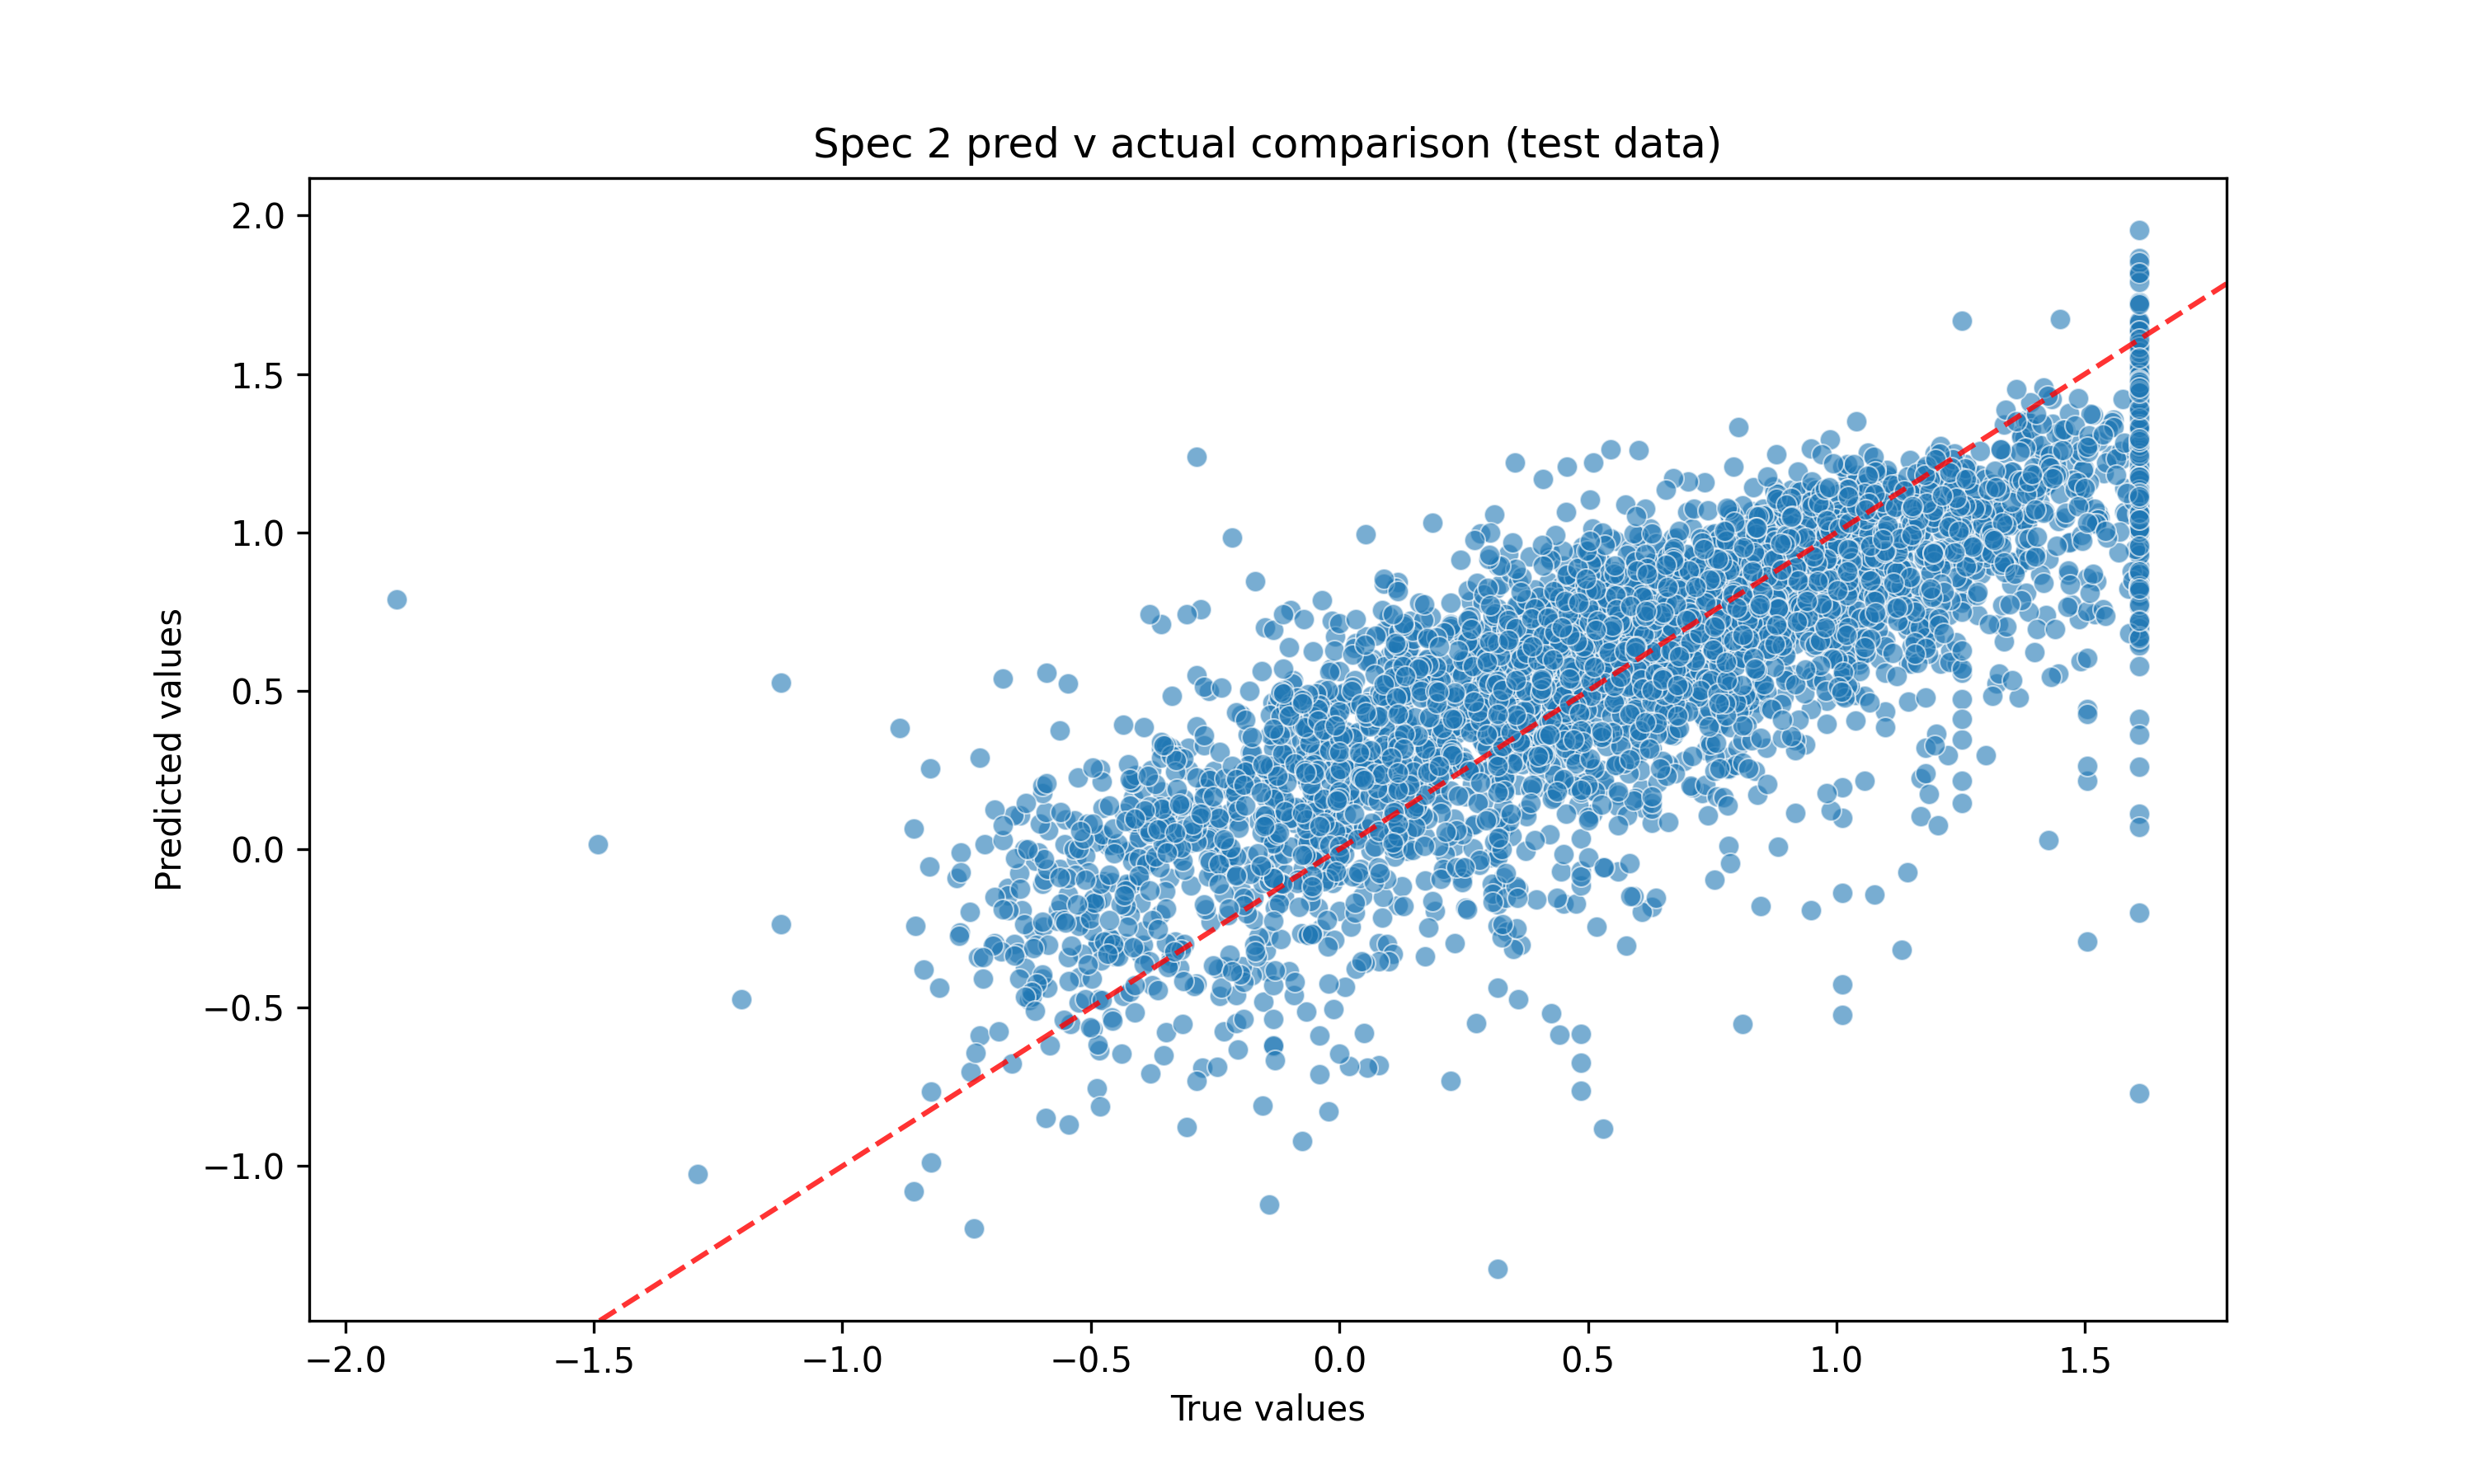
\includegraphics[width=0.8\linewidth]{plots/Spec_2_pred_v_actual_test.png}
\caption{Predicted vs. True Values (Test Data)}
\end{figure}

\begin{figure}[h]
\centering
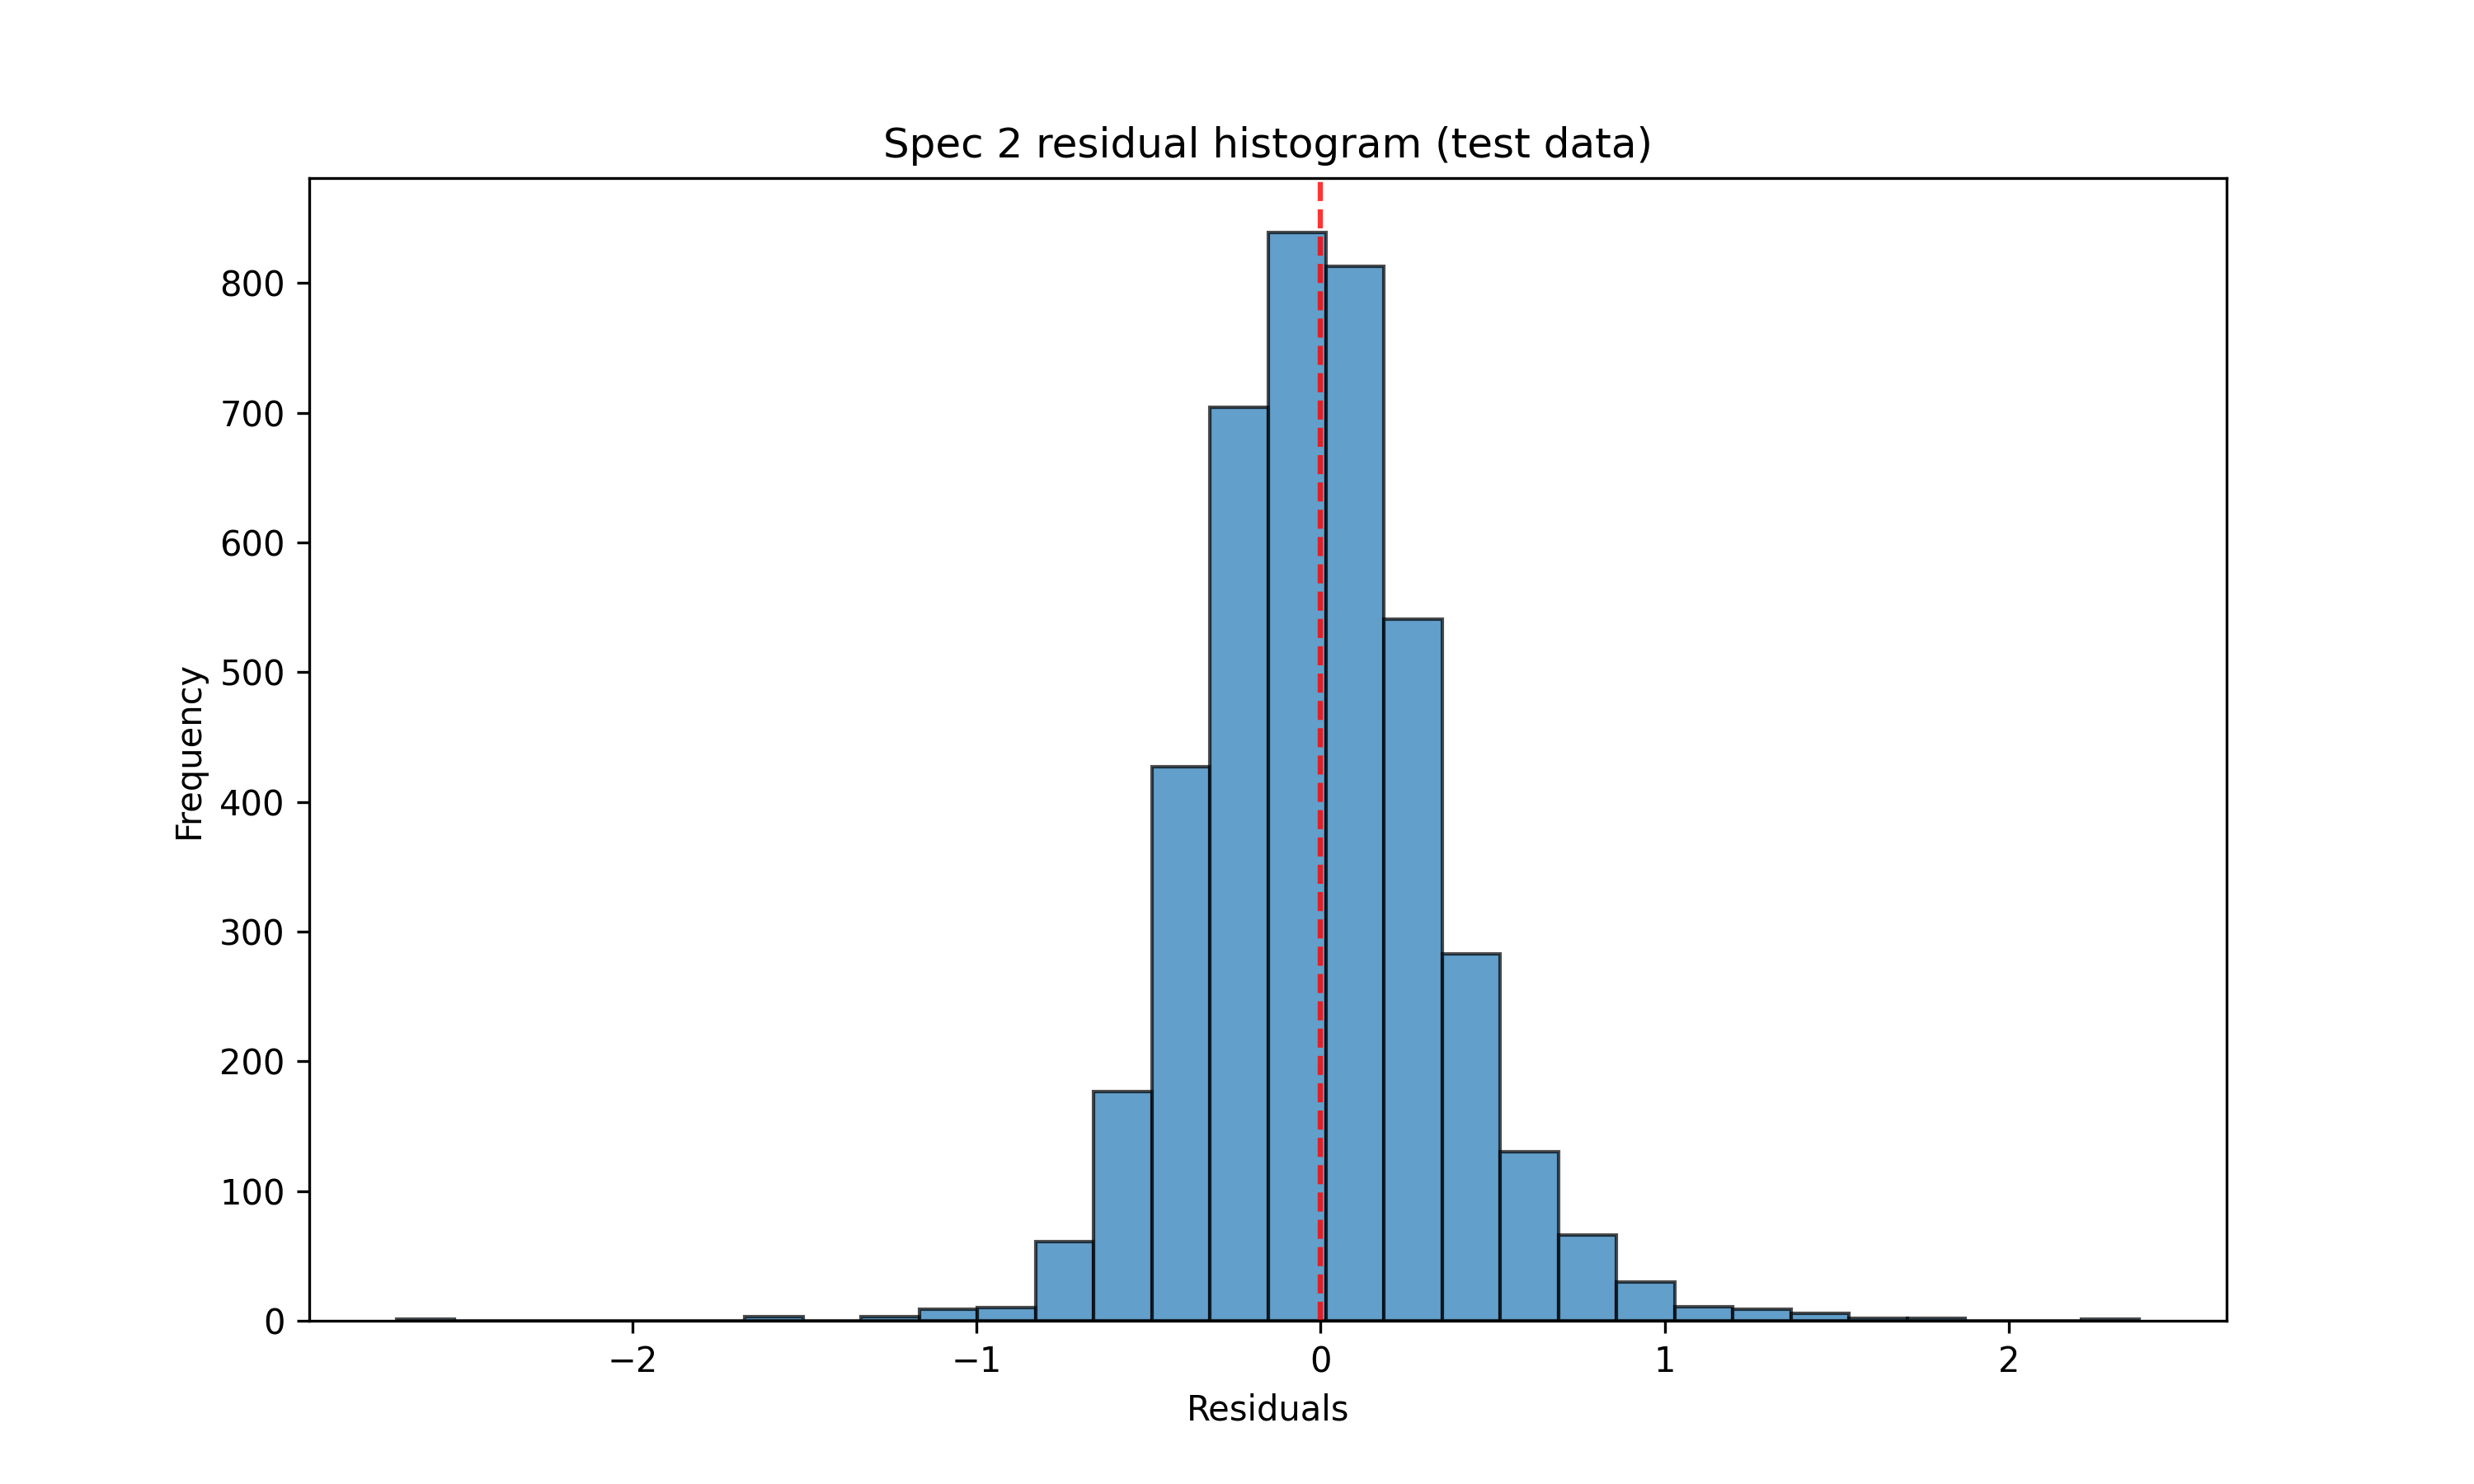
\includegraphics[width=0.8\linewidth]{plots/Spec_2_residual_hist_test.png}
\caption{Residual Distribution (Test Data)}
\end{figure}

\subsubsection{Ridge Regression}
Ridge regression was applied with ($\alpha=1.0$). The results were virtually identical to standard linear regression, suggesting minimal multicollinearity concerns in the dataset. Plots not included for brevity, you can see them in the repo if desired.

\begin{table}[h]
\centering
\begin{tabular}{lcc}
\hline
Metric & Training Data & Test Data \\
\hline
R² & 0.629 & 0.615 \\
MSE & 0.120 & 0.122 \\
RMSE & 0.347 & 0.350 \\
MAE & 0.264 & 0.265 \\
\hline
\end{tabular}
\caption{Performance metrics for ridge regression}
\end{table}

\subsection{Variable Importance}
The most significant predictor was, by a  wide margin, \texttt{log\_medinc} (log median income), which I find consistent with my experience, confirming something is not horribly wromg. Geographic coordinates (\texttt{Latitude} and \texttt{Longitude}) showed moderate predictive power, while housing characteristics (\texttt{AveRooms}, \texttt{HouseAge}) contributed modestly to the model, with (\texttt{AveBedrms}) having the most impact from that family.

\subsection{Interpretation}
The residual distribution appears approximately normal, suggesting no bias issues. The similarity between training and test performance indicates reasonable generalization, though the moderate R² values suggest unobserved geographic or structural factors may influence housing prices beyond the available predictors. There is no mechanism to make causal claims with this analysis.


%%%%%%%%%%%%%%%%%%%%%%%%%%%%%%%%%%
\section{Classification Analysis}
\subsection{Dataset Description}
The Breast Cancer Wisconsin Dataset contains 30 features computed from digitized images of fine needle aspirates of breast masses, including characteristics like radius, texture, perimeter, area, smoothness, compactness, concavity, concave points, symmetry, and fractal dimension. The target variable classifies tumors as malignant (0) or benign (1).

\subsection{Interpretation}
Two classification approaches were implemented: Support Vector Machine (SVM) with linear kernel and k-Nearest Neighbors (KNN). Features were standardized prior to modeling. My plotting function had the confusion matrixes as part of the chart before I read the assignment, but I think it is fine.

\subsection{Support Vector Machine Results}
The linear SVM did allright, correctly classifying 97.5\% of the data:

\begin{table}[h]
\centering
\begin{tabular}{l|c|}
\textbf{Training Set Performance} & \textbf{Value} \\
\hline
Accuracy & 0.989 \\
ROC AUC & 0.998 \\
Average Precision & 0.998 \\
\hline
\end{tabular}
\end{table}

\begin{table}[h]
\centering
\begin{tabular}{l|c|}
\textbf{Test Set Performance} & \textbf{Value} \\
\hline
Accuracy & 0.983 \\
ROC AUC & 0.996 \\
Average Precision & 0.998 \\
\hline
\end{tabular}
\end{table}

\begin{table}[h]
\centering
\begin{tabular}{l|c|}
\textbf{Top 3 Predictive Features} & \textbf{Coefficient} \\
\hline
mean concave points & 0.967 \\
radius error & 0.944 \\
worst fractal dimension & 0.917 \\
\hline
\end{tabular}
\end{table}


\begin{center}
\begin{tabular}{l|c|c|}
 & \textbf{Predicted Malignant} & \textbf{Predicted Benign} \\
\hline
\textbf{Actual Malignant} & 40 & 2 \\
\hline
\textbf{Actual Benign} & 2 & 70 \\
\hline
\end{tabular}
\end{center}

\begin{figure}[h]
\centering
\includegraphics[width=0.8\textwidth]{plots/svc_test_eval.png}
\caption{SVM Test Performance}
\end{figure}



Then onto the knn method; less a model and more just comparison but still does classification.
With this model, the "most important parameter" is not a relevant question, and running the training data would just match 1-to-1 and get 100\% on all metrics, so both are excluded.
I put it in a loop, and found that 8 nearest neighbors was optimal, the following are the results for that method:

\begin{table}[h]
\centering
\begin{tabular}{l|c|}
\textbf{Test Set Performance} & \textbf{Value} \\
\hline
Accuracy & 0.965 \\
ROC AUC & 0.977 \\
Average Precision & 0.976 \\
\hline
\end{tabular}
\end{table}

\begin{center}
\begin{tabular}{l|c|c|}
 & \textbf{Predicted Malignant} & \textbf{Predicted Benign} \\
\hline
\textbf{Actual Malignant} & 39 & 3 \\
\hline
\textbf{Actual Benign} & 1 & 71 \\
\hline
\end{tabular}
\end{center}

\subsection{Interpretation}
Both models demonstrate solid discriminatory power, with both achieving the same overall error rate on the testing data. The models seem to have slight differience in false positive/negative distribution, but there is too few observed errors to realy tell. The feature importance analysis reveals that morphological characteristics related to tumor boundary irregularity (concave points, radius error) and structural complexity (fractal dimension) are most predictive of malignancy.

The minimal performance drop from training to test sets indicates good generalization without overfitting. The high AUC and average precision scores confirm both models effectively distinguish malignant from benign cases across probability thresholds.

\begin{figure}[h]
\centering
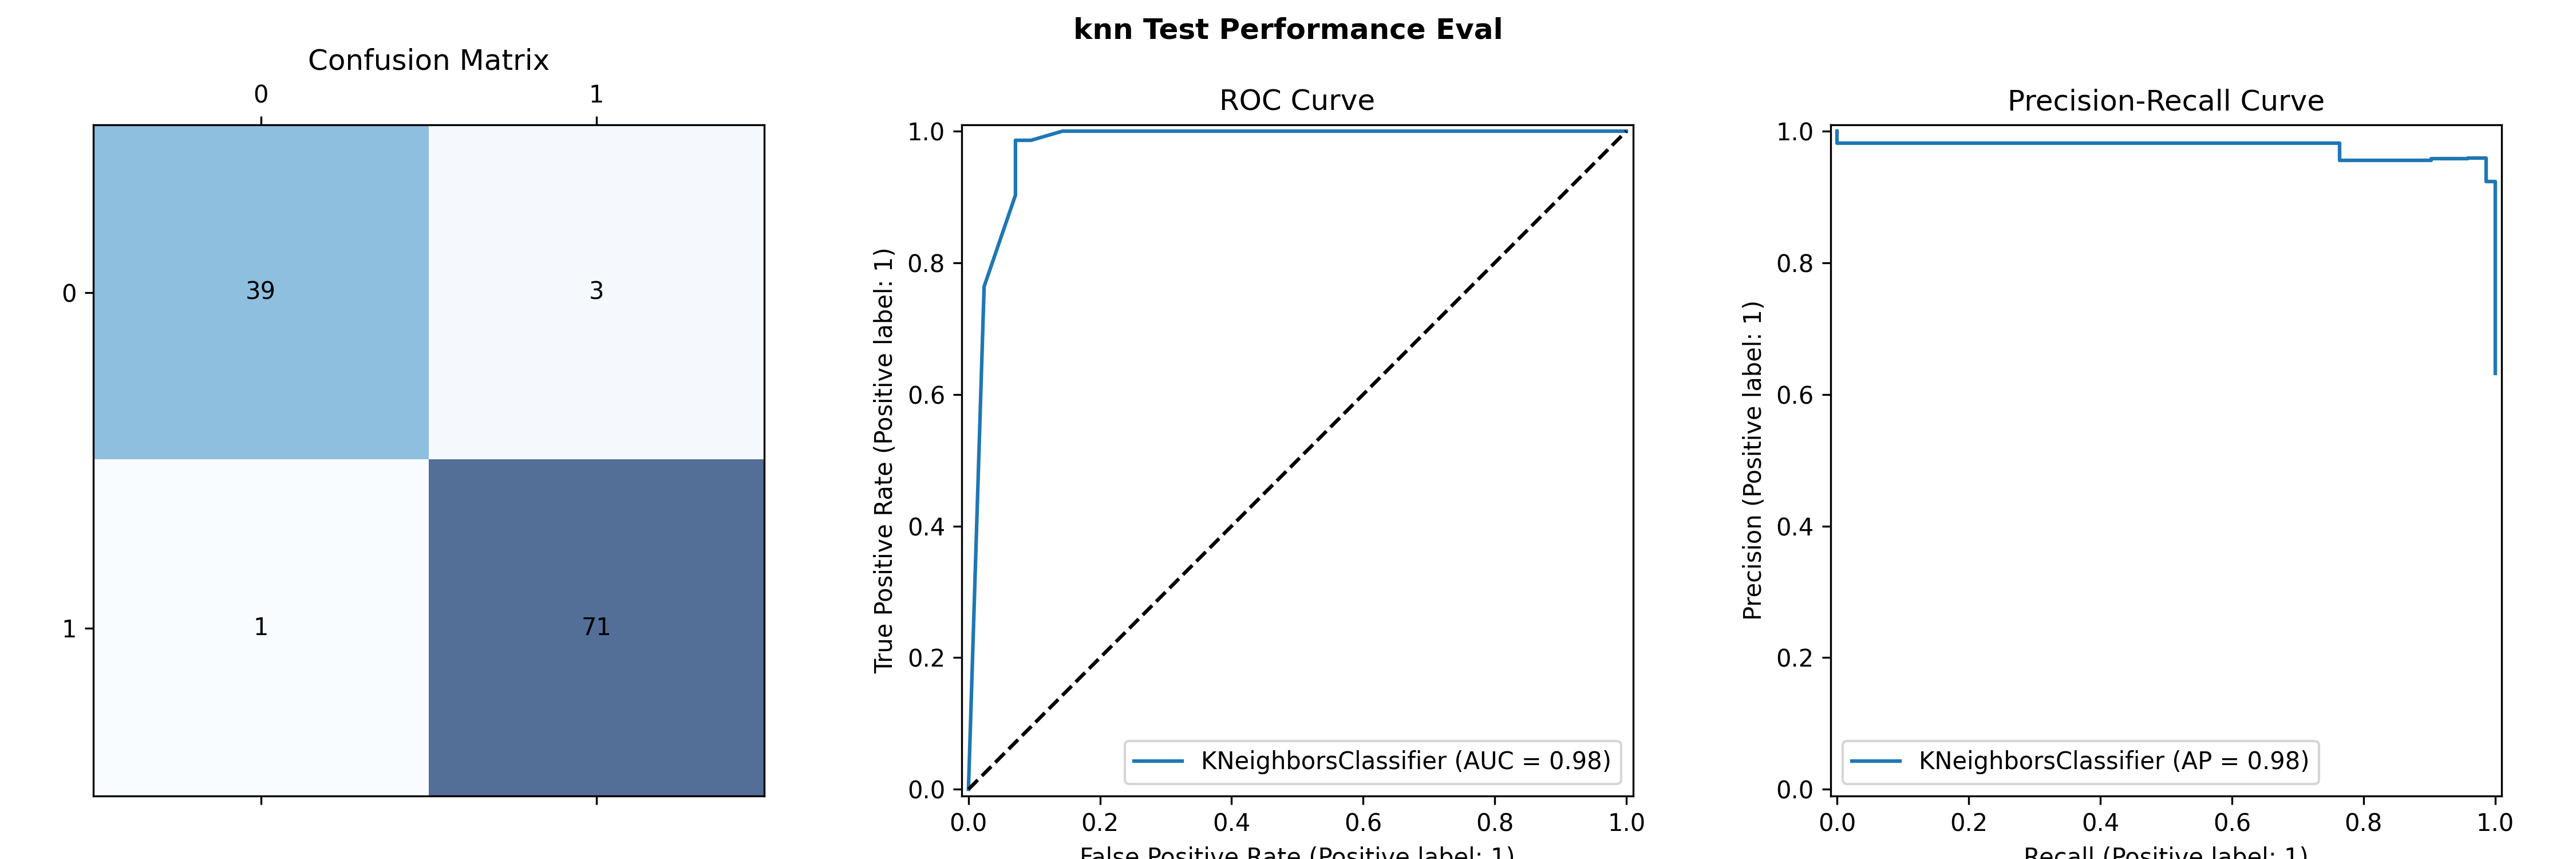
\includegraphics[width=0.8\textwidth]{plots/knn_training_eval.png}
\caption{KNN Training Performance}
\end{figure}


\end{document}
